\newpage

\section{Theoretical Background}

This chapter gives the theoretical background necessary to understand the Virtual Private Network technologies employed in this lab. We cover the fundamentals of VPNs, the specific architectures of SoftEther VPN, and the security protocols that enable the secure communication over untrusted networks.

\subsection{Virtual Private Networks (VPNs)}

Virtual Private Networks are network security solutions that provide connectivity utilizing shared infrastructure while maintaining properties typically offered in private networks. VPNs create secure communication channels over potentially untrusted networks by implementing various security mechanisms at different layers of the network stack.\\

\noindent
\textbf{Core VPN Properties:}

\noindent
A VPN must provide some essential properties to enable secure communication:

\begin{itemize}
    \item \textbf{Data Confidentiality:} Encryption algorithms protect data content from unauthorized access during transmission over public networks.
    
    \item \textbf{Data Integrity:} Cryptographic hash functions and message authentication codes ensure that data has not been modified during transmission.
    
    \item \textbf{Authentication:} Both peer authentication (verification of communicating endpoints's identities) and data origin authentication are essential for secure VPN operation.
    
    \item \textbf{Access Control:} VPN policies determine which traffic is permitted and how it needs to be processed.
    
    \item \textbf{Anti-Replay Protection:} Sequence numbers and time stamps prevent malicious replay of previously captured packets.
\end{itemize}

\noindent
\textbf{VPN Classification:}

\noindent
VPNs can be classified based on their method of implementation and the network layers at which security is enforced. The layers considered in this lab are:

\begin{itemize}
    \item \textbf{Network Layer VPNs:} Operate at the IP layer (L3), e.g. IPSec-based ones
    \item \textbf{Transport Layer VPNs:} Implement security at L4, e.g. TLS/SSL VPNs
\end{itemize}

\subsection{SoftEther VPN Architecture}

SoftEther VPN represents a unique approach to VPN deployment with a unified platform to support multiple VPN protocols simultaneously \cite{softether_official}. This feature of multi-protocol support enables straightforward comparison and evaluation of different VPN technologies in a single deployment.

\begin{figure}[H]
\centering
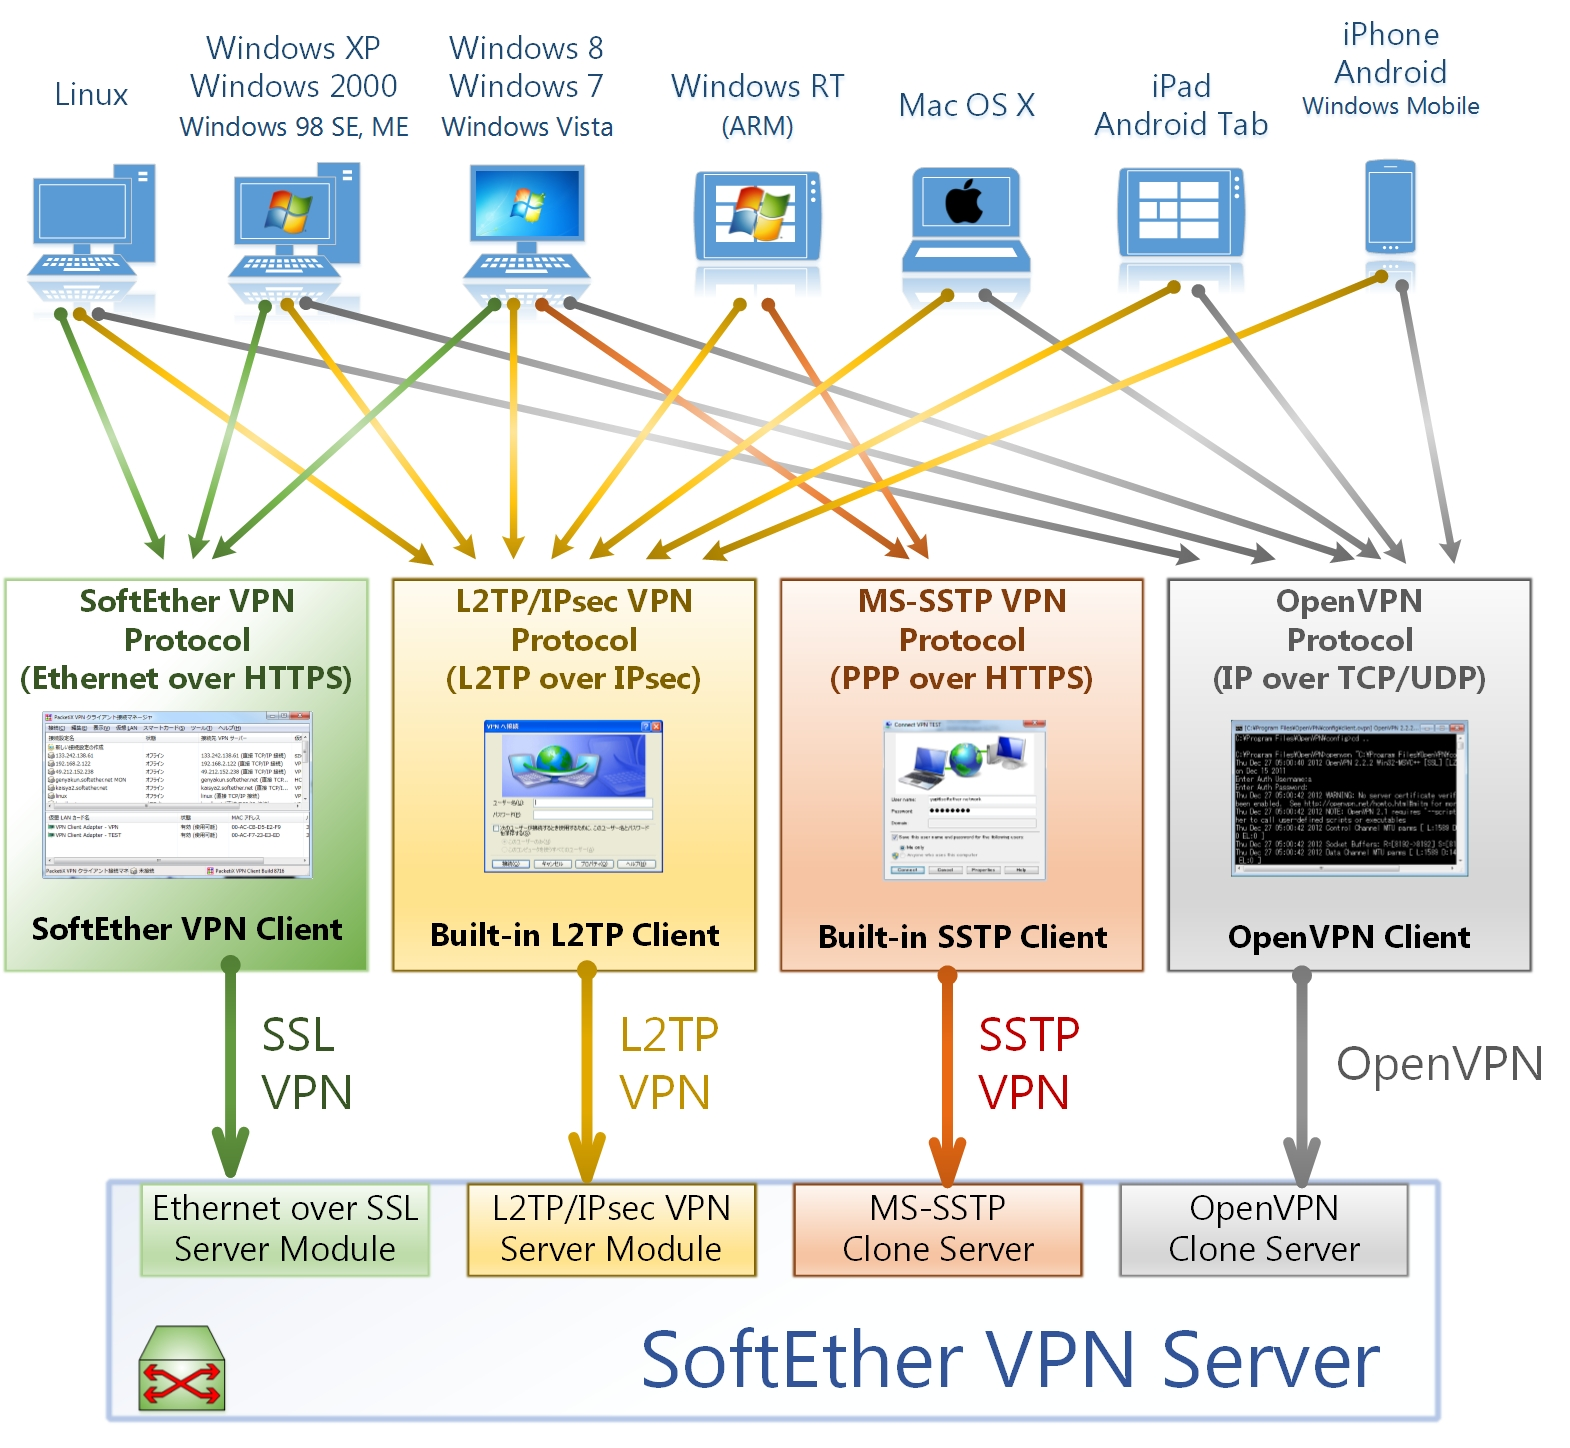
\includegraphics[width=0.4\textwidth]{../resources/Images/SoftEther_VPN_Architecture.jpg}
\caption{SoftEther VPN Multi-Protocol Architecture}
\label{fig:softether_architecture}
\end{figure}

As indicated in Figure \ref{fig:softether_architecture}, SoftEther VPN's architecture reflects its adaptability in the sense of offering Multiple client operating systems and VPN protocols. The figure explains how different hosts with different operating systems can connect to a single SoftEther VPN Server using different VPN protocols:

\begin{itemize}
    \item \textbf{SoftEther VPN Protocol:} Ethernet over HTTPS Proprietary protocol
    \item \textbf{L2TP/IPSec VPN Protocol:} Common L2TP over IPSec implementation
    \item \textbf{MS-SSTP VPN Protocol:} Microsoft's Secure Socket Tunneling Protocol using PPP over HTTPS
    \item \textbf{OpenVPN Protocol:} SSL/TLS-based VPN using IP over TCP/UDP
\end{itemize}

\noindent
\\
\textbf{Multi-Protocol Support:}

\noindent
SoftEther VPN's architecture relies on \textit{protocol abstraction}, where different VPN protocols are realized as modules within a common framework. The key protocols that we will use in this lab are:

\begin{itemize}
    \item \textbf{IPSec Support:} Built in support for both AH (Authentication Header) and ESP (Encapsulating Security Payload) protocols in tunnel mode
    \item \textbf{SSL/TLS Support:} Built-in TLS server compatible with OpenVPN clients and other SSL VPN solutions
\end{itemize}

\noindent
\textbf{Virtual Hub Architecture:}

\noindent
The core of SoftEther VPN is the Virtual Hub concept, which acts as a virtual Ethernet switch. This architecture facilitates the aggregation of multiple VPN sessions of different protocols, provides strong routing and bridging capabilities, and accomodates centralized policy enforcement and logging. Building complex network topologies, including both site-to-site networks and remote access networks, is also supported by the Virtual Hub and thus is a valuable component of SoftEther VPN applications.

\noindent
\\
\textbf{SecureNAT Functionality:}

\noindent
SoftEther VPN comes with a Built-in NAT (Network Address Translation) and DHCP server feature named SecureNAT, which is employed to make it easy to set up VPN clients by

\begin{itemize}
    \item Automatically assigning IP addresses to VPN clients
    \item Providing DNS resolution services
    \item Providing Internet access for VPN clients through NAT
\end{itemize}

\subsection{IPSec Protocol Suite}

Internet Protocol Security (\textbf{IPSec}) is a suite that provides security at the IP layer by adding headers to IP packets \cite{rfc4301}. It may operate in transport mode (only securing payload) or tunnel mode (encapsulating the entire packet). IPSec implementations have been the subject of extensive cryptographic analysis \cite{ferguson_ipsec} and are standardized by various bodies, like NIST \cite{nist_vpn_guide}.

\noindent
A key part is the \textbf{Encapsulating Security Payload} (ESP), which ensures confidentiality by encrypting packets and provides optionally integrity and authentication as well. ESP in tunnel mode, encrypts the whole IP packet, creating new IP headers for the routing. \textbf{Security Associations} (SAs) are agreements between peers that specify parameters as encryption algorithms, keys, and endpoints; each of them is associated with a Security Parameter Index (SPI). Their manual management is usually controlled by Internet Key Exchange protocols: IKEv1 (with main and aggressive modes) and IKEv2 (which both improves performance and security). In this project, IPSec (via ESP, SA, and IKE) is used to establish an encrypted network layer tunnel for situations where protection at the kernel level is required for packets.

\subsection{TLS/SSL for VPN Implementation}

\textbf{Transport Layer Security} (TLS) provides session-layer security though a handshake to agree on cipher suites \cite{rfc8446}. TLS-based VPNs (such as \textbf{OpenVPN}), tunnel arbitrary IP traffic in a TLS channel \cite{openvpn_official}, leveraging the widespread availability of TLS support and negotiable cipher suites. This approach places security processing in user space, which may be easier to deploy and customize, but with some performance trade-offs compared to kernel-based solutions.

\textbf{Layers of Authentication of TLS VPNs:} Care must be taken to distinguish between TLS handshake authentication (typically server certificate verification) and application-layer authentication occurring inside the established TLS tunnel. User credentials are transmitted as application data after the secure channel has been established, again controlling access beyond the transport-layer security.

\subsection{Client-Side VPN Technologies}

\textbf{StrongSwan (IPSec):}

\noindent
strongSwan is an open-source IPSec implementation used in this project for establishing and maintaining IPSec tunnels \cite{strongswan_official, strongswan_docs}. It supports IKEv1 and IKEv2, a cryptographic algorithm set, and other features like NAT traversal \cite{rfc3948}. It can be configured with simple files (e.g., \texttt{ipsec.conf} and \texttt{ipsec.secrets}), and it supports the Linux kernel’s IPSec stack. In our setup, strongSwan handles automatic key exchanges and maintains SAs for secure network-layer tunnels.\\

\noindent
\textbf{OpenVPN Client (TLS):}

\noindent
OpenVPN is the TLS-based client solution in this project \cite{openvpn_official, openvpn_howto}. It is based on OpenSSL for cryptography \cite{openssl_project}, supports both UDP and TCP transports, and can be configured in tun (Layer 3) or tap (Layer 2) mode. Certificate-based authentication using a certificate ensures that only authorized endpoints connect. OpenVPN’s user-space implementation supports flexible scripting hooks and logging, so it is easily adapted to custom remote-access applications in the lab.

\subsection{Comparative Analysis Framework}

Having theoretical knowledge of the differences between IPSec and TLS implementations, provides the basis for effective comparison:

\begin{itemize}
    \item \textbf{Architecture Differences:} IPSec is implemented at the network layer (typically in kernel space), whereas TLS-based VPNs run in user space at the session layer.
    
    \item \textbf{Performance Considerations:} IPSec generally has lower overhead with kernel integration; TLS-based VPNs offer more flexibility but may have more user space processing.
    
    \item \textbf{Deployment Complexity:} IPSec configurations may be more complex but follow broadly enstablished standards, while TLS-based VPNs like OpenVPN are more likely to have simpler initial setup and greater customizability.
    
\end{itemize}


This conceptual foundation establishes the necessary knowledge for understanding the actual application and comparison of SoftEther VPN's multi-protocol capabilities in subsequent parts of this lab activity.